%%
%% This is file `sample-authordraft.tex',
%% generated with the docstrip utility.
%%
%% The original source files were:
%%
%% samples.dtx  (with options: `authordraft')
%% 
%% IMPORTANT NOTICE:
%% 
%% For the copyright see the source file.
%% 
%% Any modified versions of this file must be renamed
%% with new filenames distinct from sample-authordraft.tex.
%% 
%% For distribution of the original source see the terms
%% for copying and modification in the file samples.dtx.
%% 
%% This generated file may be distributed as long as the
%% original source files, as listed above, are part of the
%% same distribution. (The sources need not necessarily be
%% in the same archive or directory.)
%%
%% The first command in your LaTeX source must be the \documentclass command.
\documentclass[sigconf %,authordraft
]{acmart}
\usepackage[T1]{fontenc}
%\usepackage{lmodern}
%\usepackage[utf8]{inputenc}
%\usepackage{amsfonts}
\usepackage{eurosym}
%\usepackage{amsmath}
%\usepackage{amssymb}
%\usepackage{booktabs}

%\usepackage{epsfig} 
%\usepackage{cite}
\usepackage{color}
\usepackage{multirow}
\usepackage{mathtools}
%\usepackage{subfig}

    
\usepackage[para]{footmisc}

\usepackage[inline]{enumitem}

\newtheorem{task}{Task}

%%% \squishlist definition, list with reduced margins
\newcommand{\squishlist}{
 \begin{list}{$\bullet$}
  { \setlength{\itemsep}{0pt}
     \setlength{\parsep}{3pt}
     \setlength{\topsep}{3pt}
     \setlength{\partopsep}{0pt}


     \setlength{\leftmargin}{1em}
     \setlength{\labelwidth}{1em}
     \setlength{\labelsep}{0.5em} } }

%
%\newcommand{\squishlisttwo}{
% \begin{list}{$\bullet$}
%  { \setlength{\itemsep}{0pt}
%    \setlength{\parsep}{0pt}
%    \setlength{	opsep}{0pt}
%    \setlength{\partopsep}{0pt}
%    \setlength{\leftmargin}{2em}
%    \setlength{\labelwidth}{1.5em}
%    \setlength{\labelsep}{0.5em} } }

\newcommand{\squishend}{
  \end{list}  }
%\renewcommand{\baselinestretch}{0.99}

%% \BibTeX command to typeset BibTeX logo in the docs
\AtBeginDocument{%
  \providecommand\BibTeX{{%
    \normalfont B\kern-0.5em{\scshape i\kern-0.25em b}\kern-0.8em\TeX}}}

%% Rights management information.  This information is sent to you
%% when you complete the rights form.  These commands have SAMPLE
%% values in them; it is your responsibility as an author to replace
%% the commands and values with those provided to you when you
%% complete the rights form.
\copyrightyear{2020}
\acmYear{2020}
\setcopyright{acmcopyright}
\acmConference[WSDM '20]{The Thirteenth ACM International Conference on Web Search and Data Mining}{February 3--7, 2020}{Houston, TX, USA}
\acmBooktitle{The Thirteenth ACM International Conference on Web Search and Data Mining (WSDM '20), February 3--7, 2020, Houston, TX, USA}
\acmPrice{15.00}
\acmDOI{10.1145/3336191.3371860}
\acmISBN{978-1-4503-6822-3/20/02}

%%
%% Submission ID.
%% Use this when submitting an article to a sponsored event. You'll
%% receive a unique submission ID from the organizers
%% of the event, and this ID should be used as the parameter to this command.
%%\acmSubmissionID{123-A56-BU3}

%%
%% The majority of ACM publications use numbered citations and
%% references.  The command \citestyle{authoryear} switches to the
%% "author year" style.
%%
%% If you are preparing content for an event
%% sponsored by ACM SIGGRAPH, you must use the "author year" style of
%% citations and references.
%% Uncommenting
%% the next command will enable that style.
%%\citestyle{acmauthoryear}

%%
%% end of the preamble, start of the body of the document source.
\begin{document}
\fancyhead{}
%%
%% The "title" command has an optional parameter,
%% allowing the author to define a "short title" to be used in page headers.
%\title[Searching for Entities with Numerical Constraint in Text]{Searching for Entities with Numerical Constraint in Text}
\title{Entities with Quantities: Extraction, Search, and Ranking}
%%
%% The "author" command and its associated commands are used to define
%% the authors and their affiliations.
%% Of note is the shared affiliation of the first two authors, and the
%% "authornote" and "authornotemark" commands
%% used to denote shared contribution to the research.
\author{Vinh Thinh Ho}
%\authornote{Both authors contributed equally to this research.}
\email{hvthinh@mpi-inf.mpg.de}
%\orcid{1234-5678-9012}
%\author{G.K.M. Tobin}
%\authornotemark[1]
%\email{webmaster@marysville-ohio.com}
\affiliation{%
  \institution{Max Planck Institute for Informatics}
%  \streetaddress{P.O. Box 1212}
  \city{Saarbr\"ucken}
%  \state{Ohio}
%  \postcode{43017-6221}
  \country{Germany}
}

\author{Koninika Pal}
\email{kpal@mpi-inf.mpg.de}

\affiliation{%
  \institution{Max Planck Institute for Informatics}
  \city{Saarbr\"ucken}
  \country{Germany}
}

\author{Niko Kleer}
\email{nkleer@mpi-inf.mpg.de}
\affiliation{%
  \institution{Max Planck Institute for Informatics}
  \institution{htw saar}
  \city{Saarbr\"ucken}
  \country{Germany}
}

\author{Klaus Berberich}
\email{kberberi@mpi-inf.mpg.de}
\affiliation{%
  \institution{Max Planck Institute for Informatics}
    \institution{htw saar}
  \city{Saarbr\"ucken}
  \country{Germany}
}

\author{Gerhard Weikum}
\email{weikum@mpi-inf.mpg.de}
\affiliation{%
  \institution{Max Planck Institute for Informatics}
  \city{Saarbr\"ucken}
  \country{Germany}
}

%%
%% By default, the full list of authors will be used in the page
%% headers. Often, this list is too long, and will overlap
%% other information printed in the page headers. This command allows
%% the author to define a more concise list
%% of authors' names for this purpose.
\renewcommand{\shortauthors}{Ho, et al.}

%%
%% The abstract is a short summary of the work to be presented in the
%% article.

\begin{abstract}
	
 
Quantities are more than numeric values. They represent measures for entities, expressed in numbers with associated units. 
Search queries often include quantities, such as athletes who ran 200m under 20 seconds or companies with quarterly revenue above \$2 Billion. Processing such queries requires
understanding the quantities, where capturing the surrounding context is an essential part of it. 
Although modern search engines or QA systems handle entity-centric queries well, they consider numbers and units as simple keywords, and therefore fail to understand the condition (less than, above, etc.), the unit of interest (seconds, dollar, etc.), and the context of the quantity (200m race, quarterly revenue, etc.) 
As a result, they cannot generate the correct candidate answers.  
In this work, we demonstrate a prototype QA system, called Qsearch, 
that can handle advanced queries with quantity constraints using the common cues present in both query and the text sources.
%Quantities appear in search queries in numerous forms: 
%to find a products within a specific price range, 
%to locate a country with an increasing GDP, to identify athletes who won multiple Olympic medals, among others.
%companies with annual revenue of at least 50 Mio USD, athletes who ran 200 meters faster than 19.5 s, electric cars with range above 400 miles, and so on.
%Processing such queries requires the understanding of numbers present in the query to capture the contextual information about the queried entities. 
%Modern search engines and QA systems
%like Google, Bing, etc. can 
%efficiently handle queries that involve entities and types, 
%which need to exploit only relational structures embedded in Web content and social media for queried entities. 
%But they fail to produce crisp answers to the queries involving numerical constraints as they disregard the reasoning %over quantitative information.
%but they often fail on properly interpreting quantities in queries and candidate answers
%when the specifics of the search condition (less than, above, etc.), the units of interest (seconds, miles, meters, etc.)
%and the context of the quantity matter (annual or quarterly revenue, etc.).
%  
%Numeric answers for such queries might appear in various sources, either structured (e.g. tables, lists), or unstructured (e.g. text), where processing unstructured text are more challenging. 
%Modern search engines like Google, Bing, etc. support queries that involve relational structures embedded in Web content and social media and can provide crisp answers to the queries or questions. However, informative quantities are usually disregarded. 
%
%Approach and  Contribution

%tackles queries with numerical constraints by harnessing quantitative  contextual information about entities from text.
%can effectively answer advanced queries with quantity conditions, based on the evidence from text sources.
%Our solution is based on a deep neural network for extracting quantity-centric tuples from text sources,
%and a novel matching model to 
%retrieve and rank
%answers 
%from news articles and other web pages.

%In particular, we propose a framework for representing quantitative information, 
%an efficient deep neural network for extracting these information from textual data, 
%produce 
%for given numerical queries. 
%Experiments 
%on real-world data 
%demonstrate the effectiveness of Qsearch on benchmark queries collected by crowdsourcing.

\end{abstract}

%%
%% The code below is generated by the tool at http://dl.acm.org/ccs.cfm.
%% Please copy and paste the code instead of the example below.
%%
%\begin{CCSXML}
%<ccs2012>
% <concept>
%  <concept_id>10010520.10010553.10010562</concept_id>
%  <concept_desc>Computer systems organization~Embedded systems</concept_desc>
%  <concept_significance>500</concept_significance>
% </concept>
% <concept>
%  <concept_id>10010520.10010575.10010755</concept_id>
%  <concept_desc>Computer systems organization~Redundancy</concept_desc>
%  <concept_significance>300</concept_significance>
% </concept>
% <concept>
%  <concept_id>10010520.10010553.10010554</concept_id>
%  <concept_desc>Computer systems organization~Robotics</concept_desc>
%  <concept_significance>100</concept_significance>
% </concept>
% <concept>
%  <concept_id>10003033.10003083.10003095</concept_id>
%  <concept_desc>Networks~Network reliability</concept_desc>
%  <concept_significance>100</concept_significance>
% </concept>
%</ccs2012>
%\end{CCSXML}

%\ccsdesc[500]{Computer systems organization~Embedded systems}
%\ccsdesc[300]{Computer systems organization~Redundancy}
%\ccsdesc{Computer systems organization~Robotics}
%\ccsdesc[100]{Networks~Network reliability}

%%
%% Keywords. The author(s) should pick words that accurately describe
%% the work being presented. Separate the keywords with commas.

\keywords{Semantic Search, Question Answering, Information Extraction,
%Numeric 
Quantities}

%% A "teaser" image appears between the author and affiliation
%% information and the body of the document, and typically spans the
%% page.

%\begin{teaserfigure}
%  \includegraphics[width=\textwidth]{sampleteaser}
%  \caption{Seattle Mariners at Spring Training, 2010.}
%  \Description{Enjoying the baseball game from the third-base
%  seats. Ichiro Suzuki preparing to bat.}
%  \label{fig:teaser}
%\end{teaserfigure}

%%
%% This command processes the author and affiliation and title
%% information and builds the first part of the formatted document.
\maketitle

%!TEX root = ../main.tex

\section{Introduction}\label{sec:intro}


%Quantities, such as \$2B, 40 mpg or 19.19 s, are more than mere numbers; they express measures 
%like revenue, fuel consumption or time in a race with a numeric value and a corresponding unit. 
%The occurrence of a quantity in the text or a table of a web page is associated with an entity and interpretable only with the surrounding context. 
%The interpretation of these quantities is only possible through the associated entities and in context. 
%For example, in the sentence “BMW i8 costs about 138k Euros in Germany and has a battery range between 50 and 60 km.”, the quantity e138.000 (after normalization) refers to the price of the car model BMW i8, and the quantity interval [50,60]km denotes the range for that car (note that this is in electric mode only as this is a hybrid car).

%\noindent \textbf{Motivation.} Quantities appeared in the text or a table carry significant information about associated entities. Such quantities express more than a numeric value, can only be interpreted with the local context.
%For instance, in the sentence like \textit{``Tesla model S costs about \$ 99k
%in USA''},
%the quantity \$ 99K indicates the cost of the car model in dollar. 
%In a question answering system quantities can be a part of the answer for a query about an entity, e.g., ``Cost of Telsa S'', or it can be a part of the question itself, e.g., ``electric cars with price less than \$100K''.

\noindent \textbf{Motivation.} Search engines have gone a long way towards understanding
entities and their types in online contents and user queries,
by learning information extraction and 
leveraging their knowledge graphs \cite{DBLP:journals/cacm/NoyGJNPT19}.
For example, a query about \textit{``Bezos's net worth''}
returns the direct answer 113.5 Bio. USD by recognizing
the entity Jeff Bezos.
Likewise, a query with a type description like \textit{``athletes who won 200m olympics''}
returns a crisp list of entities, including Usain Bolt and others.

These capabilities for semantic search \cite{DBLP:journals/ftir/BastBH16, DBLP:conf/rweb/BastS18, DBLP:conf/ecir/GarigliottiB18}
%cite survey articles on semantic search here
%perhaps include one paper on QA 
have limitations, though.
One of them is the limited understanding of {\em quantities},
that is, quantitative measures of entities with a value and a unit, e.g.,
the personal wealth of a person, the annual
revenue of a company, the time of a 200m race's winner,
the fuel consumption of a car, and so on.
Looking up quantities for given entities is straightforward
and well supported. However, evaluating search conditions
about quantities is beyond the abilities of today's search engines. %, which requires .
Consider example queries such as:

\begin{itemize}
	\item CEOs with a net worth of more than 100 Billion dollars
	\item Athletes who ran 200m under 20 seconds
	\item Hybrid cars with a battery range above 50 km
\end{itemize}

%\squishend

Depending on the values in these queries and the way the units
are specified, major search engines occasionally return good results for
some of the queries. 
For example, the third query, with the twist that the unit is
changed to miles, returns a short list of car models ranked
by electric range, however all these are from a list of a single web page.
Changing the condition of the query from 50 km to 45 km returns a different list where all results
are incorrect (their electric range is lower than 45 miles).
If we change the value to 57, the search engine
falls back to the ten-blue-links mode and returns web pages
rather than entities.
The underlying reason for these deficiencies is that the search
engines do not understand quantities; instead they merely
match tokens that denote numbers and units as if they were keywords.
The occasional cases with good results are, by and large, accidental
(drawing from many high-quality lists and tables within web pages).




%1 par approach: Qsearch in a nutshell
\noindent \textbf{Proposed Approach.} The prototype system presented in this demo paper, called {\em Qsearch},
is an approach to overcome the outlined limitations.
Qsearch supports queries about entity types with search conditions
about quantities. The queries can take the form of keywords, telegraphic phrases
or full-fledged questions. The above examples can be handled by Qsearch.
Each produces ranked lists of entity-level results with evidence sentences
that the quantity condition is satisfied.
Measures within the scope of the prototype include financial quantities
(e.g., company revenues or earnings or prices of company acquisitions),
physical and technical measures of devices (e.g., range or fuel consumption
of cars, battery capacity of mobiles, energy consumption of data centers),
times and distances in sport competitions, and more.

%1 par on Qsearch methodology
Qsearch is based on three main components (see \cite{HoISWC2019} for full details).
First, text corpora are processed with a neural method for extracting
quantities, the entities to which they refer, and informative cue words from
their joint context, which are represented in the form of triples $(e,q, X)$ - \textit{(entity, quantity, context)}, called \textit{Qfact}. 
For instance, from the text \textit{``Tesla S costs 65k Euros in Germany''}, we extract Qfact: $(\textit{Tesla S}; \textit{\euro 65.000};\{\textit{costs, Germany}\})$.
Second, a query is decomposed into \textit{entity type}, \textit{quantity condition} and
important \textit{context} cue words, which are also casted into a triple $(t^*,q^*, X^*)$, called \textit{Qquery}. 
For example, query \textit{``Cars with price less than \euro 35,000 in Germany''} is modeled as Qquery: $(\textit{car}; < \hspace{-0.25em} \textit{\euro 35.000}; \{\textit{price, Germany}\})$. The query processing matches Qquery against
extracted Qfacts from text snippets.
Third, the query results are judiciously ranked using language models
or other criteria (e.g., entity prominence or quantity value).

%Quantities are common in search queries, for example to find a product within a specific price range,  cars or mobile phones with desired technical or environmental properties, or athletes who ran a race in a certain time. 
% When a user issues a quantity search query, such as \textit{``Hybrid cars with price under 35,000 Euros''}, 
 %and battery range above 100 km
% she expects the search engine to understand the quantities and to return relevant answers as a list of entities instead of documents.
%The relevant answer here is a list of cars that are ``less than 35,000 Euros'' and ``battery range more than 100km''. 
%However, Internet search engines treat quantities largely as strings ignoring their values and unit of measurements. As a result, they cannot handle numeric comparisons, they miss out on units
%or scale factors (such as ``k'' in ``138k''), do not know about
%necessary conversions between units,  and ultimately fail.
%The exceptional cases where search engines 
%(incl. vertical product search) provide 
%support for coping with quantities are money and date,
%but this is achieved by specialized techniques and 
%fairly limited. 
%\input{tables/kg_stats}
%One would hope that semantic search over knowledge graphs (KG) like DBpedia
%, Yago or Wikidata goes further,
%but they provide a very low coverage of quantitative facts; 
%but their coverage of quantitative facts is very limited and most literals, apart from dates, are merely represented as strings.
%; e.g., battery capacity of the BMW i3 is shown as the string
%\textit{``i3 94 A·h: 33 kWh lithium-ion battery''} in DBpedia.
%Important properties for cars, like fuel consumption, CO2 emission, etc. are not covered at all.


%display size for mobile phones are represented by number without any associated unit in DBpedia. 
%%The length of the Mercedes-Benz O405 is shown as \textit{``11.1 m''} 
%The weight of the racing car Williams FW07 is shown as \textit{``: 585 kg''} 
%%in DBpedia 
%-- again just a string that is useless for queries with comparisons 
%like vehicles with \textit{``length more than 10 meters''} or \textit{``length above 30 feets''}.
%like cars with \textit{``weight more than 500 kilograms''} or \textit{``weight above 1000 pounds''}.

%in either DBpedia or Wikidata.
%though these informations are mentioned in additional comments in form of text. 
 %Table \ref{table:kg_stats} gives exemplary numbers for the quantity coverage in Wikidata and DBpedia.
%show such low coverage of quantitative facts available in these KGs.
%For some cars like Tesla Model X, the range is shown in the form ``257$\pm$1 mile'' in Wikidata-- again just a string, while API returns simply a point value, 257 mile, rather providing the range that is useless for queries with comparisons 
%the length of the BMW i8 is shown as ``4,689 millimeter'' in Wikidata;
%like ``range above 250 miles''
%or ``range above 400 km''.
% For example, the range of the Tesla Model X is shown as ``257$\pm$1 mile'' in Wikidata -- just a string that is useless for queries with comparisons like ``range above 250 miles'' or ``range above 400 km''; fuel consumption, CO2 emission, etc. are not covered at all.

%Moreover, question answering systems over linked data (incl. KGs)
%have rarely considered quantities in search condition, e.g., a popular benchmark for quantity queries, QALD-6-task-3~\cite{DBLP:journals/semweb/UsbeckRHCHNDU19}, contains only 6 queries with quantity conditions out of 150.

%While range, display size and personal best time are important properties for entity types car, mobile and marathon runner, respectively; these data are not available at all, or the data type is not always included. The exception is stadium capacity, but the number in this case is dimensionless, which is easier to handle.

%Several form-based search engines were created to counter this issue, such as specialized products search engines. However, these form-based search engines are tedious to use and only covers a specific class of items, normally stored in a single relational database. 

%It is complex to find the central entitiy, and 
%uantities appear in search queries in numerous forms: to find a product within a specific price range, to locate a country with an increasing GDP, to explore movies produced in a specific year, to identify athletes who won multiple Olympic medals, among others. They represent an indispensable part of the query that defines the set of the possible answers. Therefore, they necessitate special handling to understand them within their context.

%the current gap in the search engines
 %Natural language queries involving quantities are common. However, modern search engines fail to answer them. Most of the search engines are keyword-based or entity-based.

 %As a result, they treat quantities as a string ignoring their values and unit of measurements.  Moreover, search engines usually retrieve a ranked list of webpages, except for some cases at which search queries involves prominent entities or events.   


 
%\noindent \textbf{Proposed Approach.}
%We demonstrate Qsearch \cite{HoISWC2019}, an end-to-end system for answering quantity queries from text,  over a wide variety of expressive measures, to overcome
%this severe limitation of today's search engines and knowledge graphs.
%%We define our problem as follows.
%Given a quantity query and a corpus of text pages, 
%find a ranked list of entities that match the given query. 
%
%The computational framework used by Qsearch for representing quantitative information has been introduced in our previous work \cite{HoISWC2019}. In particular, we model a quantity query (Qquery \cite{HoISWC2019}) as a triple $\mathcal{Y}=(t^*,q^*, X^*)$, where 
%$t^*$ is the semantic type of the expected answers, 
%$q^*$ is a quantity-centric search condition, and 
%$X^*$ is a context conditon, a bag of words describing the connection between entity type  $t^*$ and quantity condition $q^*$. For example, for the query  \textit{``Cars with price less than \euro 35,000 in Germany''}, the triple $(t^*,q^*, X^*)$ is: $(\textit{car}; < \textit{\euro 35.000}; \{\textit{price, Germany}\})$.
%
%Analogously, we model a quantity fact (Qfact \cite{HoISWC2019}) as a triple $\mathcal{F}=(e,q, X)$, where
%$e$ is an entity, 
%$q$ is a quantity, and 
%$X$ is the context that connects entity $e$ with quantity $q$.
%For example, from the text snippet \textit{``BMW i8 costs about 138k Euros in Germany and has a battery range between 50 and 60 km.''}, we can extract two Qfacts:
%$\mathcal{F}_1: (\textit{BMW i8}; \approx\hspace{-0.25em} \textit{\euro 138.000}; \{\textit{costs, Germany}\})$
%and $\mathcal{F}_2: (\textit{BMW i8};\\ \textit{50-60 km}; \{ \textit{range, battery} \})$.
%
%
%With this representation of queries and facts, our problem has two dimensions.
%The first is to understand the content of the text snippets and extract the relevant Qfacts. The second is to match such extracted
%assertions (inevitably with noise and errors) against the Qquery
%and compute a ranked list of relevant entity answers.
%
%For the first component, 
%Qsearch employs a deep neural network
%to extract Qfacts from text, lifting textual information into semantic structures.
%Then for the second component, it utilizes a statistical matching model to retrieve a ranked list of relevant entities that answer the user's Qquery.

%We model the first component, Qfact extraction, as a Semantic Role Labeling (SRL) task \cite{DBLP:journals/coling/GildeaJ02} and devise a 
%deep learning method to label words in the sentences with relevant roles; then use these tags to extract quantity fact triples.
%%We label each word as entity, quantity or context (or other). 
%%Then we use these tags to extract quantity fact triples in form of \textit{(entity, quantity, context)}.
%For the second component, query matching, we devise a 
%novel
%matching method to retrieve 

%On the other hand, we preprocess the corpus of web documents into triples of $(E,Q,X)$, where $E$ is an entity, $Q$ is a quantity related to $E$, and $X$ is the context defining the relation between $E$ and $Q$. For example, the triple \textit{(BMW i8, \{costs, Germany\}, \euro 138.000)} corresponds to the following sentence: \textit{``The BMW i8 costs about \euro 138k in Germany.''}
 %Then, we semantically match the query to the facts we extract from the web corpus. We generate a ranked list of objects matching the query.
%challanges 
%how we do it
%We split the quantity search problem into two essential components: 
%(i)\emph{Quantity-fact extraction from text} (ii)\emph{Query matching}

%more about the approach here!

%We design a full-fledged system that answers complex quantity queries. preprocesses web content, index them, and answers complex quantity queries in an efficient manner.  Our system extracts quantity-related facts from web pages and stores them as a triple of  $(E, Q, X)$. It transforms the problem to a \emph{Semantic Role Labelling} task and employs a \emph{Deep Semantic Role Labeling (DSRL)} model to label sentences. % with $E$, $Q$, and $X$ tags.

%\subsubsection{Limitations of Prior Work.}
%\subsubsection{Outlook}
% research focused on answering quantity queries 
%recent work covering quantity extraction and fact extraction
%QA

%%%GW: this is too long for here (intro)
%Though, some of the previous work tackled, binary and n-ary quantity fact extraction~\cite{DBLP:conf/www/ErnstSW18} and semantic annotation of quantities\cite{DBLP:conf/cikm/IbrahimRW16, Ibrahim:ICDE2019}, none of them looked into how to harness these semantic annotations to answer quantity-related queries. 
%Zhang et al.~\cite{DBLP:conf/sigmod/ZhangC13} consider semantic matching of quantities on web tables, but did not give attention to quantities in natural text.  The work of Banerjee et al.~\cite{DBLP:conf/sigir/BanerjeeCR09} answers quantity consensus queries, however, they only consider binary relations and rely on hand-crafted rules. 
%State of the art retrieval models do not focus on quantity queries nor do they consider extracting quantity facts from the text. On the other hand factoid question answering (QA) systems merely function as a quantity-lookup form structured semantic knowledge. Other QA systems have been proposed to answer reading comprehension questions, however, they do not aggregate answers from multiple sources and they focus on general questions rather than quantity queries. 


%On the other hand, we employ \emph{Deep Semantic Role Labeling  (DSRL)} to extract n-ary quantity facts, and provide a robust system to process and answer quantity queries.

\noindent \textbf{Outline.}
In Section \ref{sec:system_overview}, we briefly describe the architecture of Qsearch and the approach underlying its main components. Afterwards, we illustrate the features provided by our demonstration through graphical user interface in Section \ref{sec:demo}. Finally, Section \ref{sec:related-work} mentions related work and Section \ref{sec:conclusion} concludes the paper. We make our demo available to the research community at the following URL: \textcolor{blue}{\url{https://qsearch.mpi-inf.mpg.de/}}

%The salient contributions of this work are as follows:
%\begin{itemize}
%\item We present Qsearch, a system for answering quantity queries from text.
%\item We propose a deep neural network for quantity fact extraction, and a matching model for answering quantity queries.
%\item  We present extensive experiments on benchmark queries collected by crowdsourcing.%, demonstrating the effectiveness of our approach with respect to the correctness of answers.

%\item We make code, data and a running demo available to the research community at\\{\small\url{http://anonymous-for-double-blind-review/}}.
%\end{itemize}

\section{System Overview}
\label{sec:system_overview}

Figure \ref{fig:system} 
%shows the high-level architecture of 
gives an overview of the architecture of 
Qsearch that has been introduced in our earlier work \cite{HoISWC2019}. 
%The arrows in the figure depict information flow between the different system components. 
Qsearch consists of two main phases:
\textit{Extract}
and \textit{Answer}.
 
%In this section, we demonstrate our numerical question answering system from text. In Figure \ref{fig:system}, we present a high-level architecture of our system, where the arrows depict information flow between building blocks. We split the working flow of our system into two main stages: \textit{Extract} and \textit{Answer}.

\begin{figure}[t]
\centering
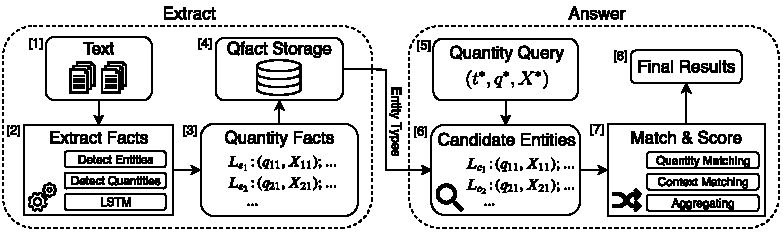
\includegraphics[width=0.5\textwidth]{figures/overview.pdf}
\caption{Overview of Qsearch \cite{HoISWC2019}.}
\label{fig:system}
\vspace{-1em}
\end{figure}
% what is the storage, how is it stored, and indexed 

\subsection{Extract}  
We preprocess to recognize named entities in the input text corpus (Block 1) using AIDA \cite{DBLP:conf/emnlp/HoffartYBFPSTTW11} system that links entity mentions
%in text are linked 
to the YAGO knowledge base \cite{DBLP:conf/www/SuchanekKW07}.
%and link them to an external knowledge base (KB).
%To achieve a better detection quality, we run NED on a per-document instead of per-sentence basis.
We also detect quantity mentions in the text and normalize them into standard units. For this, we make use of the Illinois Quantifier \cite{DBLP:journals/tacl/RoyVR15}, a state-of-the-art tool for 
recognizing quantities in text, along with some hand-crafted rules (e.g., regular expressions). 

Subsequently, we run a specifically designed Long Short Term Memory (LSTM) network to extract Qfacts in the form of triples $(e,q,X)$ from each individual preprocessed sentence (Block 2). The neural network structure has been described in our work \cite{HoISWC2019}. The main idea is that, for each quantity detected in the preprocessing step, the neural network identifies the entity to which it refers
and the relevant context tokens that express the relation between them. Figure \ref{fig:example} illustrates an example of how Qsearch extracts Qfacts from sentences. In this example, the quantity $q_1$ is mapped to the entity $e_1$ and context $\{\textit{price, Germany}\}$, whereas the quantity $q_2$ is also mapped to the entity $e_1$ but with context $\{\textit{range, battery}\}$.


After the neural-based extraction, all Qfacts having the same named entity are grouped together, so that each individual entity $e_i$ is connected with a list of quantities and contexts, expressed as $L_{e_i} = \{(q_{i1},X_{i1}),(q_{i2},X_{i2}),... \}$ (Block 3).
Entities are also linked to their semantic types from the KB, and we store these structures in a data repository in Block 4. In our implementation, Elasticsearch is used as the storage engine.

\begin{figure}[t]
\centering
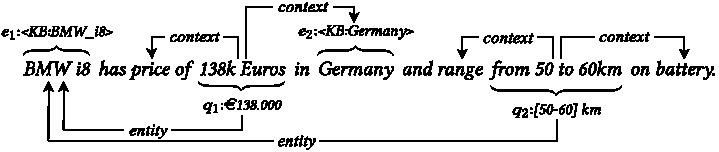
\includegraphics[width=0.5\textwidth]{figures/example_2.pdf}
\caption{Each detected quantity is linked to a corresponding entity and relevant context tokens.}
\label{fig:example}
\vspace{-1em}
\end{figure}

\subsection{Answer}
In this phase, Qqueries are answered by matching against Qfacts extracted from before. 

\noindent \textbf{Query Parsing.} In Block 5, the input questions are transformed into Qquery format $(t^*,q^*,X^*)$ by a rule-based parser. The parser uses a dictionary of YAGO types and a dictionary of quantity units to recognize the target semantic type of answers $t^*$ and the quantity condition $q^*$. Then, it includes all remaining tokens of the query (except stopwords) in the query context $X^*$ \cite{HoISWC2019}.

\noindent \textbf{Answer Matching.} First, based on the type information from the KB, a list of candidate entities $\mathcal{C} = \{c_1,c_2,...\}$ that satisfy the target type $t^*$ are retrieved from the Qfact repository, along with their quantity-context pairs $\{L_{c_1},L_{c_2},...\}$ (Block 6). Second, we perform quantity matching with the support of a list of unit conversion rules, filtering all Qfacts that do not meet the quantity condition $q^*$ (Block 7).
Finally, each candidate entity $c \in \mathcal{C}$ is assigned a score calculated based on matching contexts $X$ against $X^*$. 
%The candidate entities are ranked by their scores and returned to the user (Block 8).
Here, we make use of two context ranking models for measuring the context relevance: \textit{Kullback-Leibler divergence (KL)} and \textit{context embedding distance (ced)} (see \citep{HoISWC2019} for details).

 

%In the following Sections
%\ref{sec:extract} and \ref{sec:match}, we discuss in detail the
% Qfact extraction model and the matching and answering model, 
%respectively.

%In the remainder of this section, we discuss how each candidate entity is scored in Block 7.

\noindent \textbf{Kullback-Leibler Divergence.} The Kullback-Leibler divergence between the query context $X^*$ and the fact context $X$ is defined as:
\begin{align*}
\textit{KL}(X^*, X) &= H(X^*, X) - H(X^*) \\ &\equiv H(X^*, X) 
= -\sum_{w \in \mathcal{V}} P(w|X^*)\,\log P(w|X)
\end{align*}
where $\mathcal{V}$ is the word vocabulary, $H(X^*)$ is the entropy of $X^*$; $H(X^*, X)$ is the cross entropy between $X^*$ and $X$; and $\equiv$ is rank equivalence
(i.e., preserving order, $H(X^*)$ is omitted). 
%Since we are only interested in ranking fact contexts in response to a query context, we can omit $H(X^*)$.
The two probabilities $P(w|X^*)$ and $P(w|X)$ 
%for query context and fact context 
are estimated using Maximum Likelihood Estimation (MLE) with WordNet-based context expansion and Jelinek-Mercer smoothing to avoid zero probabilities \cite{HoISWC2019}.

% on an expanded version $X^*_E$ of $X^*$ as:
%\[P(w|X^*) = count(w \in X^*_E)/|X^*_E|\]
%To expand a query context, we resort to WordNet \cite{Miller:1995:WLD:219717.219748} and add all synonyms of the context words to it. For the fact context, we estimate the word probability $P(w|X)$ using Jelinek-Mercer smoothing 
%%to avoid zero probabilities
% as:
%\[P(w|X) = (1 - \lambda) \times count(w \in X)/|X| + \lambda \times P(w|B)\]
%This linearly combines the MLE from the fact context $X$ with the MLE obtained from a background corpus $B$. The smoothing parameter $\lambda$ (set to $\lambda=0.1$ in our system) controls the influence of the background corpus on the probability estimate. We construct the background corpus $B$ from all sentences of the entire text corpus that contain at least one quantity (total 39M sentences in our data). \\
%

%Since these two estimates are very sparse, before calculating, we expand $X^*$ and $X$ using an external resource. Moreover, a smoothing method is applied to avoid zero counts.
%\thinh{Should explain more? which resource, how to expand, which smoothing method.}

\begin{figure*}[t]
\centering
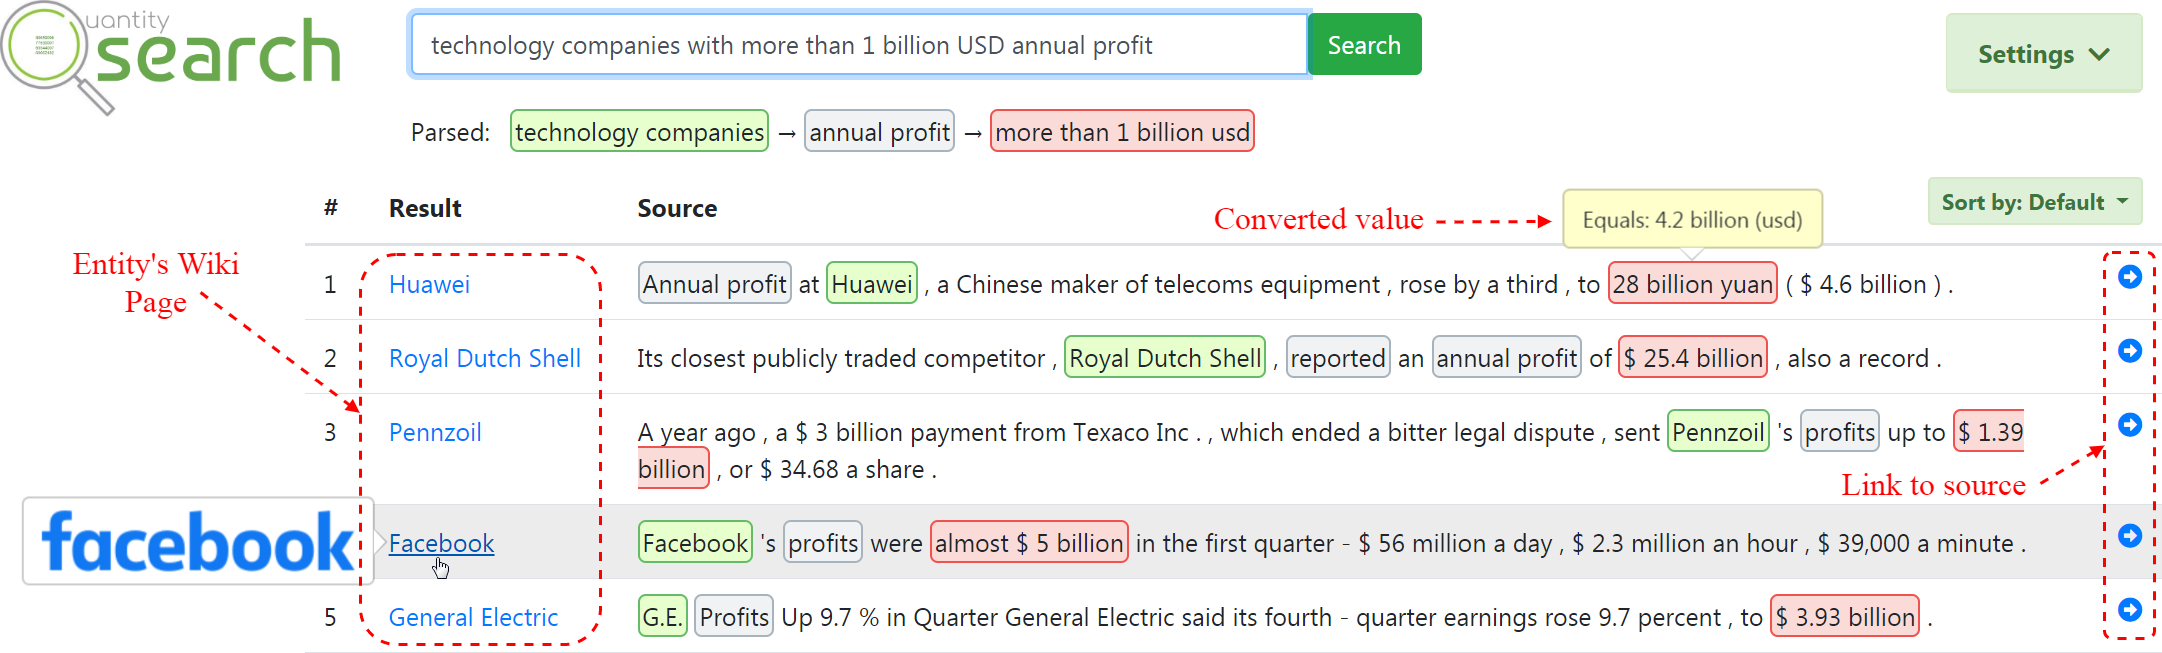
\includegraphics[width=1\textwidth]{figures/new/gui.png}
\caption{Qsearch Web interface.}
\label{fig:gui}
\vspace{-1em}
\end{figure*}

\noindent \textbf{Context Embedding Distance.}
The novel context embedding distance for measuring context relevance is defined as follows:
\[ced(X^*, X) = ded(X^* \rightarrow X) \times ded(X \rightarrow X^*)^\alpha\]
where $ded(A \rightarrow B)$ is the \textit{directed embedding distance} between two bags of words $A$ and $B$, computed as:
\[ded(A \rightarrow B) = 1 + \Bigg(\sum\limits_{u \in A} W(u)\min\limits_{v \in B}(d(u,v))\Bigg)\big/\sum\limits_{u \in A}W(u)\]
where $d(u,v)$ is the semantic distance between two words $u$ and $v$, computed using word embeddings 
%estimated from their pre-computed word embedding vectors
 \cite{DBLP:conf/emnlp/PenningtonSM14}; $W(u)$ is the importance weight of $u$; in this case, \textit{inverse document frequency (idf)} is used by Qsearch.
% (e.g., \textit{inverse document frequency (idf)}, \textit{term strength}, etc.); Qsearch uses Robertson's \textit{idf} \cite{DBLP:journals/jd/Robertson04}. 
%We use cosine distance in the Qsearch implementation, re-scaled for normalization to [0,1]. 
%In the above equation, 
%we map each word of query context $X^*$ to its closest word in the fact context $X$ in the embedding space. This scoring formula gives the same weight to every token in the query context $X^*$, which might be misleading, since they could have a different degree of importance.
%This issue is overcome by giving higher weight to important words and lower weight
%to uninformative words, using
%%we use 
%the following distance function:
%\[d(\mathcal{F}, \mathcal{Y}) = \frac{\sum\limits_{u \in X^*} W(u)\min\limits_{v \in X}(dist(u,v))}{\sum\limits_{u \in X^*}W(u)} + 1\]
%We call the above formula the 
%\textit{directed embedding distance}, $ded(X^* \rightarrow X)$,
%between query and fact contexts.
Putting into words, $ced$ consists of two parts: (1) $ded(X^* \rightarrow X)$ measures how well query context tokens match with fact context, and (2) $ded(X \rightarrow X^*)$ captures how much other terms in $X$ change its meaning, and thus, should be penalized in the total score. $\alpha \geq 0$ controls the influence of this penalty.

%\begin{example} Consider the Qquery context $X^* = \{\textit{gross, domestic, product}\}$ and two Qfact contexts $X_1 =$ \{\textit{gross, national, product}\}, $X_2 =$  \{\textit{gross, domestic, product, capita}\}. While we are more inclined to $X_1$ than $X_2$, the directed embedding distance $ded(X^* \rightarrow X_2)$ has a slightly better score than $ded(X^* \rightarrow X_1)$, as it does not penalize the word \textit{``capita''}
%(which indicates that the GDP is per capita, not the total GDP). 
%In contrast, $ded(X_1 \rightarrow X^*)$ is lower than $ded(X_2 \rightarrow X^*)$ (since \textit{``national''} is close to \textit{``domestic''}), preferring $X_1$ over $X_2$ with regard to $X^*$, which results in the desired ranking based on the context embedding distance $ced$. \qed
%\end{example}



\noindent \textbf{Entity Scoring.}
After applying entity-type and quantity filters, each entity is assigned a score from one of its linked Qfacts, which has the best context distance to the Qquery. Then, they are ranked by their scores to produce the final results (Block 8).
%In Block 7 of the system overview (Figure \ref{fig:system}), we give 
%We assign a score for each candidate entity 
%$c \in \mathcal{C}$ based on its quantity-context pairs $L_{c} = \{(q_{c1},X_{c1}),%(q_{c2},X_{c2}),... \}$. Note that after filtering based on the quantity condition, we only need %to consider context matching.
%based on one of the above context distance models and
%aggregating over the entity's quantity-context pairs as follows:
%\[\textit{score}(c \in \mathcal{C}, \mathcal{Y}) = \min\limits_{(q, X) \in L_c} d(\mathcal{F}=(c,q,X), \mathcal{Y})\]
%where $d(\mathcal{F}, \mathcal{Y})$ is either the Kullback-Leibler divergence $\textit{KL}(X^*, X)$ or the context embedding distance
%$ced(X^*,X)$.
%Each entity is assigned a score from one of its linked Qfacts, which has the best context distance to the Qquery. Note that at this time we already apply entity-type and quantity filters. Candidate entities are ranked by their scores then shown to the users (Block 8).
%So when the same candidate entity appears in multiple Qfacts, we pick the best-scoring
%Qfact context distance.
%Put differently, we rank candidate entities based on their best fact context, i.e., the one %achieving the lowest distance to the query context.

\section{Demonstration}
\label{sec:demo}

We developed a Web interface to allow users to experience our Qsearch system. Figure \ref{fig:gui} shows a screenshot of the top search results for an example quantity query.

%\noindent \textbf{Implementation Details.} // TODO (machine, language, library)



%\noindent \textbf{Input.} Qsearch allow users to type a quantity query as input. 
%% The input question is mapped into Qquery format by a rule-based parser for recognizing answer type and quantity condition; all other tokens (except stopwords) are included in the query context \cite{HoISWC2019}. The parser uses a dictionary of YAGO types and a dictionary of quantity units.
%% An alternative to this rule-based technique would be to apply the same neural extraction method to questions that we have used to extract Qfacts from text. However, the questions are easier to handle, and the rule-based parser works well. 
%To give a better search experience, we show to the users a list of top YAGO types when typing the query, along with the number of relevant entities existing in our database. Figure \ref{fig:type} illustrates an example of this feature.

\noindent \textbf{Input.} Users can provide query in natural language text as input to the system. 
%The query must include one entity type and quantity. 
To give better search experience, we guide users by showing a list of top YAGO types along with the number of relevant entities existing in our database while writing the query. Figure \ref{fig:type} illustrates this feature.

\begin{figure}[t]
\centering
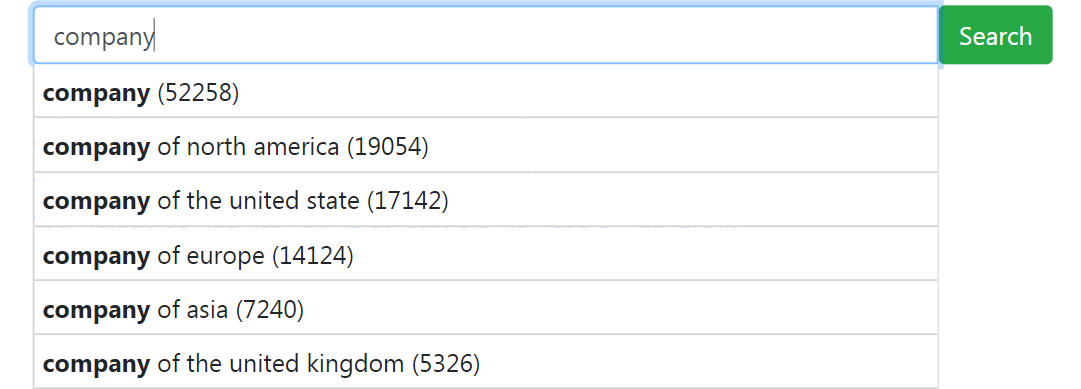
\includegraphics[width=0.5\textwidth]{figures/new/suggest.png}
\caption{Type suggestion in Qsearch.}
\label{fig:type}
\vspace{-1em}
\end{figure}

%\noindent \textbf{Output.} Qsearch processes the input query, looks for relevant entity answers and ranks them based on their distance scores to the query (using either \textit{Kullback-Leibler divergence} or \textit{context embedding distance}).

\noindent \textbf{Output.} Qsearch processes the input query and generates a ranked list of entities relevant to the input query. 
The parsed query, top answers and their entity pages (from Wikipedia) are shown to users, along with the text snippets from where the Qfacts are extracted, and the links to the original web pages (see Figure \ref{fig:gui}). For better experience, we also show the representation images of the entity answers (extracted from the entities' Wikipedia pages) to the users when they hover on the entity links. For each answer, Qsearch highlights the extracted entity, quantity and context cues of the Qfact, and also provides the converted quantity value if its unit is different from the one being asked in the query. In Table \ref{table:sample_q}, we provide some anecdotal examples of user queries and their top answers produced by Qsearch.


%!TEX root = ../main.tex
\begin{table}[t]
	\caption{Sample quantity queries and results from Qsearch.}	
	\small	
	\begin{tabular}{p{.46\textwidth}} \hline
Query \\ \hline
\textbf{Q1:} Skyscrapers with height above 1000 feet\\ 
\textbf{Q2:} Footballers with transfer cost more than 50 million Euros \\  
\textbf{Q3:} Sprinters who ran 100 meter in less than 10 seconds  \\  
%\textbf{Q4:} Companies of Europe having more than 100 thousand employees\\ \bottomrule 
	\end{tabular}
	\small
	\begin{tabular}{l| p{.08\textwidth} p{.30\textwidth}} 
	 \hline
		Query & Result & Corresponding Sentence \\ \hline
		\multirow{2}{*}{Q1}& Empire State Building & 102nd Floor Building: Empire State Building, New York Height: 1,250 feet.\\ 	\cline{2-3}	
		& Mercury City Tower & 	Eleven high-rises have already been built, among them the golden Mercury City Tower, at a height of 339 meters, the tallest skyscraper in Europe.\\ 
		\hline
		\multirow{2}{*}{Q2} & Neymar & The judge says Neymar cost at least 83.3 million euros (\$88 million), while Barcelona insists it paid 57 million euros (then \$74 million). \\ 	\cline{2-3}
		& Raheem Sterling & 	Raheem Sterling became the most expensive English footballer ever on Tuesday after joining Manchester City from Premier League rival Liverpool in a drawn-out move costing 49 million pounds (\$114 million).\\ 
		\hline
		
		\multirow{2}{*}{Q3} & Andre De Grasse & Andre De Grasse, a 20-year-old from Markham, Ont., has run the 100 metre in under 10 seconds three times this year. \\ 	\cline{2-3}
		& Walter Dix & 		Walter Dix, a Florida State sprinter, ran the 100 meter dash in 9.93 seconds, the fastest time in the world this year and the second fastest ever by a collegian.\\ 
		\hline
%		\multirow{2}{*}{Q4}		& Tyco International & 	Based in Bermuda, with headquarters in Exeter, N.H., Tyco has 240,000 employees and makes everything from security systems to syringes.\\ 
%\cline{2-3}

		
% & Volkswagen Group & Volkswagen Group, with its multiple brands, has more than 600,000 employees but the cuts will mainly fall on its 120,000-strong German work force. \\  	
%		\hline
	\end{tabular}	
	\label{table:sample_q}
	\vspace{-1em}
\end{table}


%\noindent \textbf{Text Corpora.} We use a large collections of news articles, compiled from two real world datasets: the \textit{STICS} project \cite{DBLP:conf/sigir/HoffartMW14} with news from 2014 to 2018 (containing 5.84M documents), 
%and the \textit{New York Times} archive
%%\cite{nyt}
% %5843811 + 1765538
%with news from 1986 to 2008 (containing 1.77M documents). These datasets are also used in our earlier work \cite{HoISWC2019}. Moreover, we also integrate a collection of Wikipedia web pages in this demonstration (containing 5.78M documents). In total, our text copora consist of 13.39M documents.
%\noindent \textbf{Explore Qsearch.} Our demonstration system answers quantity queries based on information from three large collections of text documents. Two real world news corpora are used: the \textit{STICS} project \cite{DBLP:conf/sigir/HoffartMW14} (containing 5.84M documents) and the \textit{New York Times} archive (containing 1.77M documents)
\noindent \textbf{Exploration of underlying data sources.} Qsearch answers quantity queries based on information from three large collections of text documents - two real-world news corpora, the \textit{STICS} project \cite{DBLP:conf/sigir/HoffartMW14} (containing 5.84M documents) and the \textit{New York Times} archive \cite{nyt} (containing 1.77M documents), and a collection of web pages from the English Wikipedia\footnote{\url{https://meta.wikimedia.org/wiki/Data\_dump\_torrents\#English\_Wikipedia}}(containing 5.78M documents). In total, our text data consists of 13.39M documents. By default, Qsearch uses all three collections to generate answers. However, we allow users to change this setting (see Figure \ref{fig:settings}) in order to narrow down their search on specific text collections. As the characteristic of news articles is quite different from Wikipedia articles, using both types of text collections as underlying input data allows Qsearch to answer a wide range of quantity queries. For example, information about finance or sport domain can be found all over the news articles and also in Wikipedia, but answers for queries on geological objects (e.g., glaciers with length more than 100 km) are mainly covered only by Wikipedia articles. 
%; these two are also used in our earlier work \cite{HoISWC2019}. Moreover, we also integrate a collection of web pages from English Wikipedia\footnote{\url{https://meta.wikimedia.org/wiki/Data\_dump\_torrents\#English\_Wikipedia}} in this demonstration (containing 5.78M documents). In total, our text data consists of 13.39M documents. 

\noindent \textbf{Exploration of answer generation methods.} Qsearch employs different ranking models as mentioned in Section~\ref{sec:system_overview} to rank the entity answers and shows top confident results to the users. 
In the default configuration, Qsearch uses the \textit{context embedding distance (ced)} as the ranking model, with the penalty factor $\alpha = 3$ (as in \cite{HoISWC2019}), and shows top 20 answers. 
%Qsearch looks for the results in the text documents and shows top 20 most confident entity answers to the users. 
\begin{figure}[t]
\centering
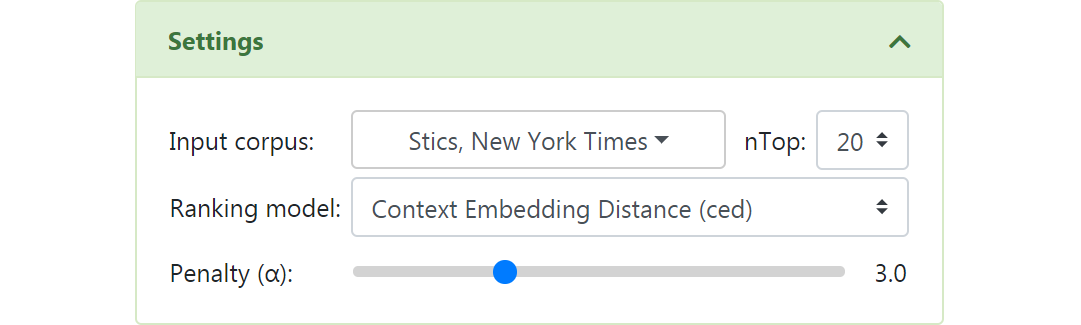
\includegraphics[width=0.5\textwidth]{figures/new/settings.png}
\caption{Qsearch options.}
\label{fig:settings}
\vspace{-1em}
\end{figure}
We provide a flexible interaction to the system by allowing users to modify these search settings (as shown in Figure \ref{fig:settings}) to explore the answer generation methods. 
Here, users can adjust the number of retrieved results (10, 20, 30, 40 or 50) or change the underlying ranking model (\textit{context embedding distance} or \textit{KL-divergence}) and its parameter. Additionally, Qsearch provides further exploration with a secondary ranking criterion, where top retrieved answers can be re-ranked either by quantity value (after normalization), or by entity prominence (based on view count of entities' Wiki pages).
This secondary ranking criterion can be set using \textit{``Sort by''} button in Figure \ref{fig:gui}.
% We provide two different secondary ranking criteria:
% to re-rank the retrieved top entity answers; 






%!TEX root = ../main.tex

\section{Related Work}
\label{sec:related-work}

%%%GW: keep this concise
%%% if we discuss QA at length, it suggests that these prior works are highly relevant and we should have compared to them

%\noindent \textbf{Question Answering.} 
%Many advanced factoid-based Question Answering (QA) systems have been developed, covering the both major paradigms in QA, IR-based QA on text corpora \cite{DBLP:conf/acl/WangN15, DBLP:conf/emnlp/YangYM15} and knowledge-based QA\cite{ DBLP:conf/coling/BaoDYZZ16, DBLP:conf/ecctd/Sanchez-Azqueta17}, or fusing them both \cite{DBLP:conf/acl/DasZRM17,DBLP:conf/emnlp/SunDZMSC18}, in order to handle complex compositional queries in natural language. Diverging from traditional open-domain QA, many recently developed QA systems \cite{DBLP:journals/corr/WestonBCM15,DBLP:conf/acl/RajpurkarJL18} address the reading comprehension task that requires understanding and reasoning of natural language.  However, none of these QA systems can efficiently handle processing and reasoning of quantitative information. 
%A few state-of-the-art works\cite{DBLP:conf/cikm/JiaARSW18} focus explicitly the reasoning of temporal constraints in questions, and most of the previous works can support mainly the counting-based numeric queries. In this work, we aim to generalize the processing of quantitative information over varied numerical constraints exploiting deep semantic role labeling. Limited number of numeric relations in the Knowledge is an important bottle neck for processing quantities, and recently has been addressed in\cite{DBLP:conf/aaai/MadaanMMRS16}. Unlike our quantity-specific context extraction model, the authors presented NumberTron which aims to extract triplets for specific numeric relations from textual corpora. 
%Tapping into semi-structured resources from Web, QEWT\cite{DBLP:conf/kdd/SarawagiC14} harnesses ambiguous and imprecise numbers in web tables and improve the performance of quantity-seeking queries.   
%KP: discussion about WikiTableQuestions ?

%%%%%%%%%%QA over knowledge graphs and other linked data sources has received great attention over the
%%%%%%%%%%last years; see \cite{DBLP:conf/rweb/UngerFC14,DBLP:journals/kais/DiefenbachLSM18} for surveys.
%%%%%%%%%%State-of-the-art methods 
%%%%%%%%%%(e.g., \cite{DBLP:conf/acl/YihCHG15,DBLP:conf/cikm/BastH15,DBLP:conf/acl/XuRFHZ16,DBLP:conf/www/AbujabalRYW18,DBLP:journals/pvldb/ZhengYZC18}) 
%%%%%%%%%%translate questions into
%%%%%%%%%%SPARQL queries, bridging the gap between
%%%%%%%%%%question vocabulary and the terminology
%%%%%%%%%%of the underlying data by means of
%%%%%%%%%%templates and/or learning from
%%%%%%%%%%training collections of question-answer pairs.
%%%%%%%%%%Benchmarks like the long-standing 
%%%%%%%%%%QALD series and other competitions
%%%%%%%%%%have shown great advances along these lines
%%%%%%%%%%\cite{DBLP:journals/semweb/UsbeckRHCHNDU19}.
%%%%%%%%%%However, these benchmark tasks hardly
%%%%%%%%%%contain any quantity queries of the kind
%%%%%%%%%%addressed here, they are mostly about quantity lookup.
%%%%%%%%%%% (even in QALD-6-task-3, only 6 out of 150 questions are of this kind, others are mostly about quantity lookup).
%%%%%%%%%% Note that look-ups of 
%%%%%%%%%%quantity attributes of qualifying entities
%%%%%%%%%%(e.g., Jeff Bezos's net worth, 10 richest people, or fastest sprinter over 100m)
%%%%%%%%%%are of a different nature, as they do not
%%%%%%%%%%contain quantity comparisons between query
%%%%%%%%%%and data (e.g., worth more than 50 million USD,
%%%%%%%%%%running faster than 9.9 seconds).
%%%%%%%%%%Moreover, the scope and diversity of the benchmark queries is necessarily restricted to relatively
%%%%%%%%%%few numeric properties, as knowledge graphs
%%%%%%%%%%hardly capture quantities in their full extent (with value and unit properly
%%%%%%%%%%separated and normalized). This is our motivation to tap
%%%%%%%%%%into text sources with more extensive coverage.
%%%%%%%%%%
%%%%%%%%%%QA over text has considered a wide range
%%%%%%%%%%of question types (e.g., \cite{DBLP:conf/emnlp/Yang0ZBCSM18,DBLP:conf/acl/GardnerC18,DBLP:conf/acl/ChenFWB17}), but there
%%%%%%%%%%is again hardly any awareness of quantity queries.
%%%%%%%%%%Keyword search, including
%%%%%%%%%%telegraphic queries, with quantity conditions
%%%%%%%%%%have been considered by 
%%%%%%%%%%\cite{DBLP:conf/emnlp/JoshiSC14}, and have been applied
%%%%%%%%%%to web tables \cite{DBLP:journals/pvldb/PimplikarS12,DBLP:conf/kdd/SarawagiC14}. 
%%%%%%%%%%%The approaches pursued in that context
%%%%%%%%%%%cannot be carried over to our setting
%%%%%%%%%%%where the data input is arbitrary natural language text.
%%%%%%%%%%\cite{DBLP:conf/sigir/BanerjeeCR09} and
%%%%%%%%%%its follow-up work \cite{DBLP:conf/kdd/SarawagiC14}
%%%%%%%%%%focused on
%%%%%%%%%%a specific kind of quantity query, namely,
%%%%%%%%%%retrieving and aggregating numerical values
%%%%%%%%%%associated with an attribute of a given entity
%%%%%%%%%%(e.g., Bezos's net worth or GDP of India).
%To this end, 
%learning-to-rank techniques over value distributions
%were developed to
%counter the uncertainty in the retrieved values,
%where web pages often contain crude estimates
%and lack exact values.
%In contrast to our setting, that work did not
%consider quantities in search conditions. 
%and did not
%require inferring units and entities to which
%quantities refer.



%\noindent \textbf{Information Extraction.}
%Recognizing and extracting numeric expressions
%from text has been addressed using
%techniques like CRFs and LSTMs 
%(e.g., \cite{DBLP:conf/aaai/MadaanMMRS16,DBLP:conf/acl/SahaPM17,DBLP:conf/sigir/AlonsoS18}).
%However, this alone does not turn numbers
%into interpretable quantities, with units
%and proper reference to the entity with
%that quantity. Only few works attempted
%to canonicalize quantities by mappings
%to hand-crafted knowledge bases 
%of measures \cite{DBLP:conf/cikm/IbrahimRW16}, but these efforts are
%very limited in scope.
%The special case of temporal expressions
%has received substantial attention
%(e.g., \cite{DBLP:series/synthesis/2016Strotgen}), but this solely covers dates
%as measures.
%
%Most related to our approach are the works
%of \cite{DBLP:conf/kdd/SarawagiC14} and \cite{DBLP:journals/tacl/RoyVR15}.
%The former used probabilistic context-free grammars
%to infer units of quantities, but focused specifically
%on web tables as inputs.
%The latter extended semantic role labeling (see below)
%to extract quantities and their units from
%natural language sentences.
%Neither of these can be readily applied
%to extracting quantities and their reference entities
%from arbitrary textual inputs.
%
%\noindent \textbf{Semantic Role Labeling.} Semantic role labeling (SRL) has been intensively researched
%as a building block for many 
%NLP tasks \cite{DBLP:journals/coling/GildeaJ02}.
%%Question Answering frameworks \cite{DBLP:conf/emnlp/ShenL07, DBLP:journals/coling/SurdeanuCZ11}, as well as, in other NLP tasks, such as Information Extraction \cite{DBLP:conf/kcap/ChristensenMSE11, DBLP:conf/naacl/StanovskyMZD18}, Machine translations \cite{DBLP:conf/coling/LiuG10}, in order to exploit the semantic representation of the predicate-argument structure of a sentence in a language. 
%Given a verb phrase of a sentence
%viewed as a central predicate, 
%%the SRL task is to assign different pre-defined roles of the verb in the sentence. 
%SRL identifies phrases that are assigned to
%pre-defined roles to form a frame-like
%predicate-arguments structure.
%%Generally, SRL \cite{DBLP:journals/coling/GildeaJ02, DBLP:conf/conll/KoomenPRY05} is considered as a classification task based on syntactic features of sentences and often uses labeled corpus, such as PropBank \cite{DBLP:journals/coling/PalmerKG05}, FrameNet \cite{DBLP:journals/lre/Baker12}. 
%%
%%Instead of relying on fine-tuned syntactic features of sentences, many recent literature consider word embeddings as one of the key features to learn SRL model using different  neural network methods \cite{DBLP:conf/acl/ZhouX15, DBLP:conf/acl/HeLLZ17a, DBLP:conf/emnlp/FitzGeraldTG015}. 
%Modern SRL methods make use of pre-computed
%word embeddings and employ deep neural networks
%for role filling (e.g., \cite{DBLP:conf/acl/ZhouX15, DBLP:conf/acl/HeLLZ17a, DBLP:conf/emnlp/FitzGeraldTG015}).
%%
%%Task1 of this work addresses conceptually similar to the SRL task. However, we map a sentence to a general semantic representation based on different quantity-specific roles for a given numeric value from the sentence. Hence, the characteristics of these roles differ from the predicate-argument roles where verbs are technically considered as predicates. In order to learn our quantity-specific SRL model, we employ word-embedding based deep SRL model \cite{DBLP:conf/acl/HeLLZ17a}.
%Our approach differs from this state-of-the-art SRL,
%as we are not primarily focused on the verb-phrase
%predicate, but consider the numeric quantity in a sentence
%as the pivot and aim to capture quantity-specific roles.
%
%%%%GW: need to trim the following
%To support exploration of quantitative facts in financial reports, \cite{Lamm2018QSRLA} proposed a 
%semantic representation for quantity-specific roles.
%% and discuss possibilities to utilize the shallow semantic parsing to develop their proposed framework. 
%%In the similar direction, in order to solve the elementary school math problems, 
%\cite{DBLP:journals/tacl/RoyVR15} devised a quantity representation as an additional component of
%an SRL method, which is part of the Illinois Curator software suite.
%% to reason about numbers in natural language. 
%%
%%Our SRL model represents a simplified version of their proposed semantic roles. For example, the roles \textit{entity}, \textit{value}, \textit{unit}, and \textit{resolution} are respectively similar to the roles  \textit{THEME}, \textit{VALUE with SIGN}, \textit{UNIT}, and \textit{MANNER} in their model. However, the  \textit{context} in our model generalizes the roles  \textit{QUANTITY}, \textit{LOCATION}, and \textit{TIME} together from QSRL model by Lamm et al. \cite{Lamm2018QSRLA}. Such generalization of semantic role makes our model simpler and helps in leveraging the problem of numerical Question Answering, addressed in this work. 
%Our approach makes use of this technique,
%%which is part of the Illinois Curator software suite,
%as a preprocessing step.
%However, we go further by 
%learning how to connect quantities with their
%respective entities and to collect relevant 
%context cues that enable our matching and
%ranking stage for query answering.


%1 par on IE
Prior work has looked into recognizing and extracting
numeric expressions from text using techniques like
CRFs and LSTMs (e.g., \cite{DBLP:conf/sigir/AlonsoS18,DBLP:journals/tacl/RoyVR15,DBLP:conf/acl/SahaPM17}).
However, this alone does not turn numbers into
interpretable quantities, as the latter require units
(e.g., MPG, kWh/100km, etc.) and proper frame of reference
(e.g., the timeframe for revenue, dosages etc.).
Only few works attempted to canonicalize quantities
by mappings to hand-crafted knowledge bases of measures \cite{DBLP:conf/cikm/IbrahimRW16},
but these efforts are very limited in scope.
The most promising one has been the work by
Sarawagi et al. on querying Web tables \cite{DBLP:conf/kdd/SarawagiC14},
with limited support for understanding measures and units.
However, this approach is tied to table data and does
not generalize to quantity search over all kinds of Web contents.

%1 par on SRL
Semantic role labeling is a slot-filling variant of information extraction,
intensively studied in NLP. Modern methods leverage word embeddings
and deep learning \cite{DBLP:conf/acl/HeLLZ17a}. 
Our extraction method uses the similar paradigm, but customizes the 
learning to our 
specific model
of Qfacts. 
%Our approach to extracting quantity structure from sentences is based
%on this paradigm, but customizes the learning to our specific model
%of Qfacts. 

%1 par on search and QA
Semantic search (e.g., \cite{DBLP:series/irs/Balog18,DBLP:journals/ftir/BastBH16, DBLP:conf/rweb/BastS18, DBLP:conf/ecir/GarigliottiB18}) has largely focused on entity-seeking queries,
where either a type description or an entity name is the starting point.
When such requests involve quantities, it is in the form of simple lookups,
for example, the net worth of Bezos or the range of the Tesla Model S.
These queries do not require any understanding of measures and
search conditions over quantities. 
The same holds for most of the work on question answering, where
natural language questions are mapped into queries over knowledge graphs
or text corpora (e.g., \cite{DBLP:conf/acl/GardnerC18,DBLP:journals/kais/DiefenbachLSM18,DBLP:conf/wsdm/HuangZLL19,DBLP:conf/emnlp/RajpurkarZLL16}).
Although some benchmarks like QALD and ComplexWebQuestions include a small
fraction of questions that mention quantities, this is almost exclusively in the form
of lookups (e.g., what is Bezos's net worth) rather than search conditions
(e.g., CEOs with net worth above 1B).



%!TEX root = ../main.tex

\section{Conclusion}
\label{sec:conclusion}

We have presented the Qsearch demo system for full-fledged support of
quantity queries, with novel approaches of information representation, information extraction and answer matching/ranking.
We capture quantities in complete extent, including measurement units, reference entities and appropriate contexts.
In the future, we plan to enhance the work further by integrating more data sources and provide better Web interface to the users.




%\paragraph*{Acknowledgements.}

%\begin{thebibliography}{10}

\bibitem{DBLP:conf/sigir/AlonsoS18}
O.~Alonso and T.~Sellam.
\newblock Quantitative information extraction from social data.
\newblock SIGIR 2018.

\bibitem{DBLP:series/irs/Balog18}
K.~Balog.
\newblock {\em Entity-Oriented Search}.
\newblock {\em The Information
  Retrieval Series}, Springer, 2018.

\bibitem{DBLP:journals/ftir/BastBH16}
H.~Bast, B.~Buchhold, and E.~Haussmann.
\newblock Semantic search on text and knowledge bases.
\newblock {\em Foundations and Trends in Information Retrieval}, 2016.

\bibitem{DBLP:conf/rweb/BastS18}
H.~Bast and N.~Schnelle.
\newblock Efficient and convenient sparql+text search: {A} quick survey.
\newblock Reasoning Web 2018.

\bibitem{DBLP:conf/acl/GardnerC18}
C.~Clark and M.~Gardner.
\newblock Simple and effective multi-paragraph reading comprehension.
\newblock ACL 2018.

\bibitem{DBLP:journals/kais/DiefenbachLSM18}
D.~Diefenbach et al.
\newblock Core techniques of question answering systems over knowledge bases: a
  survey.
\newblock {\em Knowl. Inf. Syst.}, 2018.

\bibitem{DBLP:conf/ecir/GarigliottiB18}
D.~Garigliotti and K.~Balog.
\newblock Towards an understanding of entity-oriented search intents.
\newblock ECIR 2018.

\bibitem{DBLP:conf/acl/HeLLZ17a}
L.~He et al.
\newblock Deep semantic role labeling: What works and what's next.
\newblock ACL 2017.

\bibitem{HoISWC2019}
V.~T. Ho, Y.~Ibrahim, K.~Pal, K.~Berberich, and G.~Weikum.
\newblock Qsearch: Answering quantity queries from text.
\newblock ISWC 2019.

\bibitem{DBLP:conf/sigir/HoffartMW14}
J.~Hoffart, D.~Milchevski, and G.~Weikum.
\newblock {STICS:} searching with strings, things, and cats.
\newblock SIGIR 2014.

\bibitem{DBLP:conf/emnlp/HoffartYBFPSTTW11}
J.~Hoffart et al.
\newblock Robust disambiguation of named entities in text.
\newblock EMNLP 2011.

\bibitem{DBLP:conf/wsdm/HuangZLL19}
X.~Huang et al.
\newblock Knowledge graph embedding based question answering.
\newblock WSDM 2019.

\bibitem{DBLP:conf/cikm/IbrahimRW16}
Y.~Ibrahim, M.~Riedewald, and G.~Weikum.
\newblock Making sense of entities and quantities in web tables.
\newblock CIKM 2016.

\bibitem{DBLP:journals/cacm/NoyGJNPT19}
N.~F. Noy et al.
\newblock Industry-scale knowledge graphs: lessons and challenges.
\newblock {\em Commun. {ACM}}, 2019.

\bibitem{DBLP:conf/emnlp/PenningtonSM14}
J.~Pennington, R.~Socher, and C.~D. Manning.
\newblock Glove: Global vectors for word representation.
\newblock EMNLP 2014.

\bibitem{DBLP:conf/emnlp/RajpurkarZLL16}
P.~Rajpurkar et al.
\newblock Squad: 100, 000+ questions for machine comprehension of text.
\newblock EMNLP 2016.

\bibitem{DBLP:journals/tacl/RoyVR15}
S.~Roy, T.~Vieira, and D.~Roth.
\newblock Reasoning about quantities in natural language.
\newblock {\em {TACL}} 2015.

\bibitem{DBLP:conf/acl/SahaPM17}
S.~Saha, H.~Pal, and Mausam.
\newblock Bootstrapping for numerical open {IE}.
\newblock ACL 2017.

\bibitem{nyt}
E.~Sandhaus.
\newblock The new york times annotated corpus, 2008.
	
\bibitem{DBLP:conf/kdd/SarawagiC14}
S.~Sarawagi and S.~Chakrabarti.
\newblock Open-domain quantity queries on web tables: annotation, response, and
  consensus models.
\newblock KDD 2014.

\bibitem{DBLP:conf/www/SuchanekKW07}
F.~M. Suchanek, G.~Kasneci, and G.~Weikum.
\newblock Yago: a core of semantic knowledge.
\newblock WWW 2007.

\end{thebibliography}



\bibliographystyle{abbrv}
\bibliography{references}


\end{document}
\endinput
%%
%% End of file `sample-authordraft.tex'.
